% $Header: /cvsroot/latex-beamer/latex-beamer/solutions/generic-talks/generic-ornate-15min-45min.en.tex,v 1.5 2007/01/28 20:48:23 tantau Exp $

\documentclass{beamer}
%\documentclass[mathsherif]{beamer}

% This file is a solution template for:

% - Giving a talk on some subject.
% - The talk is between 15min and 45min long.
% - Style is ornate.



% Copyright 2004 by Till Tantau <tantau@users.sourceforge.net>.
%
% In principle, this file can be redistributed and/or modified under
% the terms of the GNU Public License, version 2.
%
% However, this file is supposed to be a template to be modified
% for your own needs. For this reason, if you use this file as a
% template and not specifically distribute it as part of a another
% package/program, I grant the extra permission to freely copy and
% modify this file as you see fit and even to delete this copyright
% notice.

% Este documento ha sido realizado por los profesores Héctor Yago Corral 
% y Julia Mª Clemente Párraga del departamento de automática de la 
% universidad de Alcalá para el curso académico 2015-2016.  

\mode<presentation>
{
\usecolortheme[RGB={89,165,140}]{structure}
\usepackage[document]{ragged2e}
\usepackage{listings}
\usepackage{xcolor}
\usepackage[tikz]{bclogo}
\usepackage{cancel}

\usetheme{Warsaw}
   \definecolor{UAgrey}{RGB}{199,194,186}    
   \setbeamercolor{title}{fg=black,bg=UAgrey}
   \setbeamercolor{frametitle}{parent = palette secundary, fg = white, bg =  UAgrey}


   \setbeamercolor*{palette quaternary}{fg=white,bg=structure!50!black}
\setbeamercovered{transparent}
}

\usepackage[spanish]{babel}
\usepackage[utf8]{inputenc}
\usepackage{times}
\usepackage[T1]{fontenc}
\usepackage{lmodern}
\definecolor{myblue}{rgb}{0,0, 0.6}
\definecolor{gris}{RGB}{238,238,238}

\lstset{ 
  breaklines=true,                 
  breakatwhitespace=false,
  keepspaces=true,  
  columns=fullflexible, 
  showstringspaces=false,          
  commentstyle=\color{myblue},    
}

\newcounter{saveenumi}
\newcommand{\seti}{\setcounter{saveenumi}{\value{enumi}}}
\newcommand{\conti}{\setcounter{enumi}{\value{saveenumi}}}

\renewcommand{\lstlistingname}{Fragmento de código}% Listing -> Algorithm

\newcommand*\oldmacro{}%
\let\oldmacro\insertshorttitle%
\renewcommand*\insertshorttitle{%
  \oldmacro\hfill%
  \insertframenumber\,/\,\inserttotalframenumber}

\usepackage{tabularx}  % for 'tabularx' environment
\usepackage{ragged2e} % for \Centering macro
\newcolumntype{C}{>{\Centering\arraybackslash}X}

\title[Práctica 2 del Laboratorio de Sistemas Operativos] {Práctica 2 del Laboratorio de Sistemas Operativos}

\author[Sistemas Operativos] % (optional, use only with lots of authors)
{}

\institute[Universidad de Alcalá] % (optional, but mostly needed)
{
  %\inst{1}%
  \textcolor{structure} {\emph{\textbf{Departamento de Automática}}}\\
  Universidad de Alcalá

% - Use the \inst command only if there are several affiliations.
% - Keep it simple, no one is interested in your street address.

%\date[Short Occasion] % (optional)
%{Date / Occasion}

\vspace*{0.5cm}
\includegraphics[height=0.8cm]{../../../../transparencias/comun/uah1}
}
\date{}

\titlegraphic{
  \includegraphics[scale=0.45]{../../../../transparencias/comun/dpto}
  \hfill
  \includegraphics[scale=0.20]{../../../../transparencias/comun/gso1}
}

\subject{Talks}
\usebackgroundtemplate{\includegraphics[width=\paperwidth]{../../../../transparencias/comun/marcadeagua}}


\begin{document}

\begin{frame}
  \titlepage
\end{frame}

\section{Ciclo de creación de un programa}
	\subsection[Fases de desarrollo]{Fases de desarrollo}

	\usebackgroundtemplate{}
	\begin{frame}{Fases de desarrollo}
		\setbeamercolor{block title}{use=structure,fg=white,bg=green!75!black}
		\setbeamercolor{block body}{use=structure,fg=black,bg=green!20!white}

		\begin{figure}
			\begin{centering}
				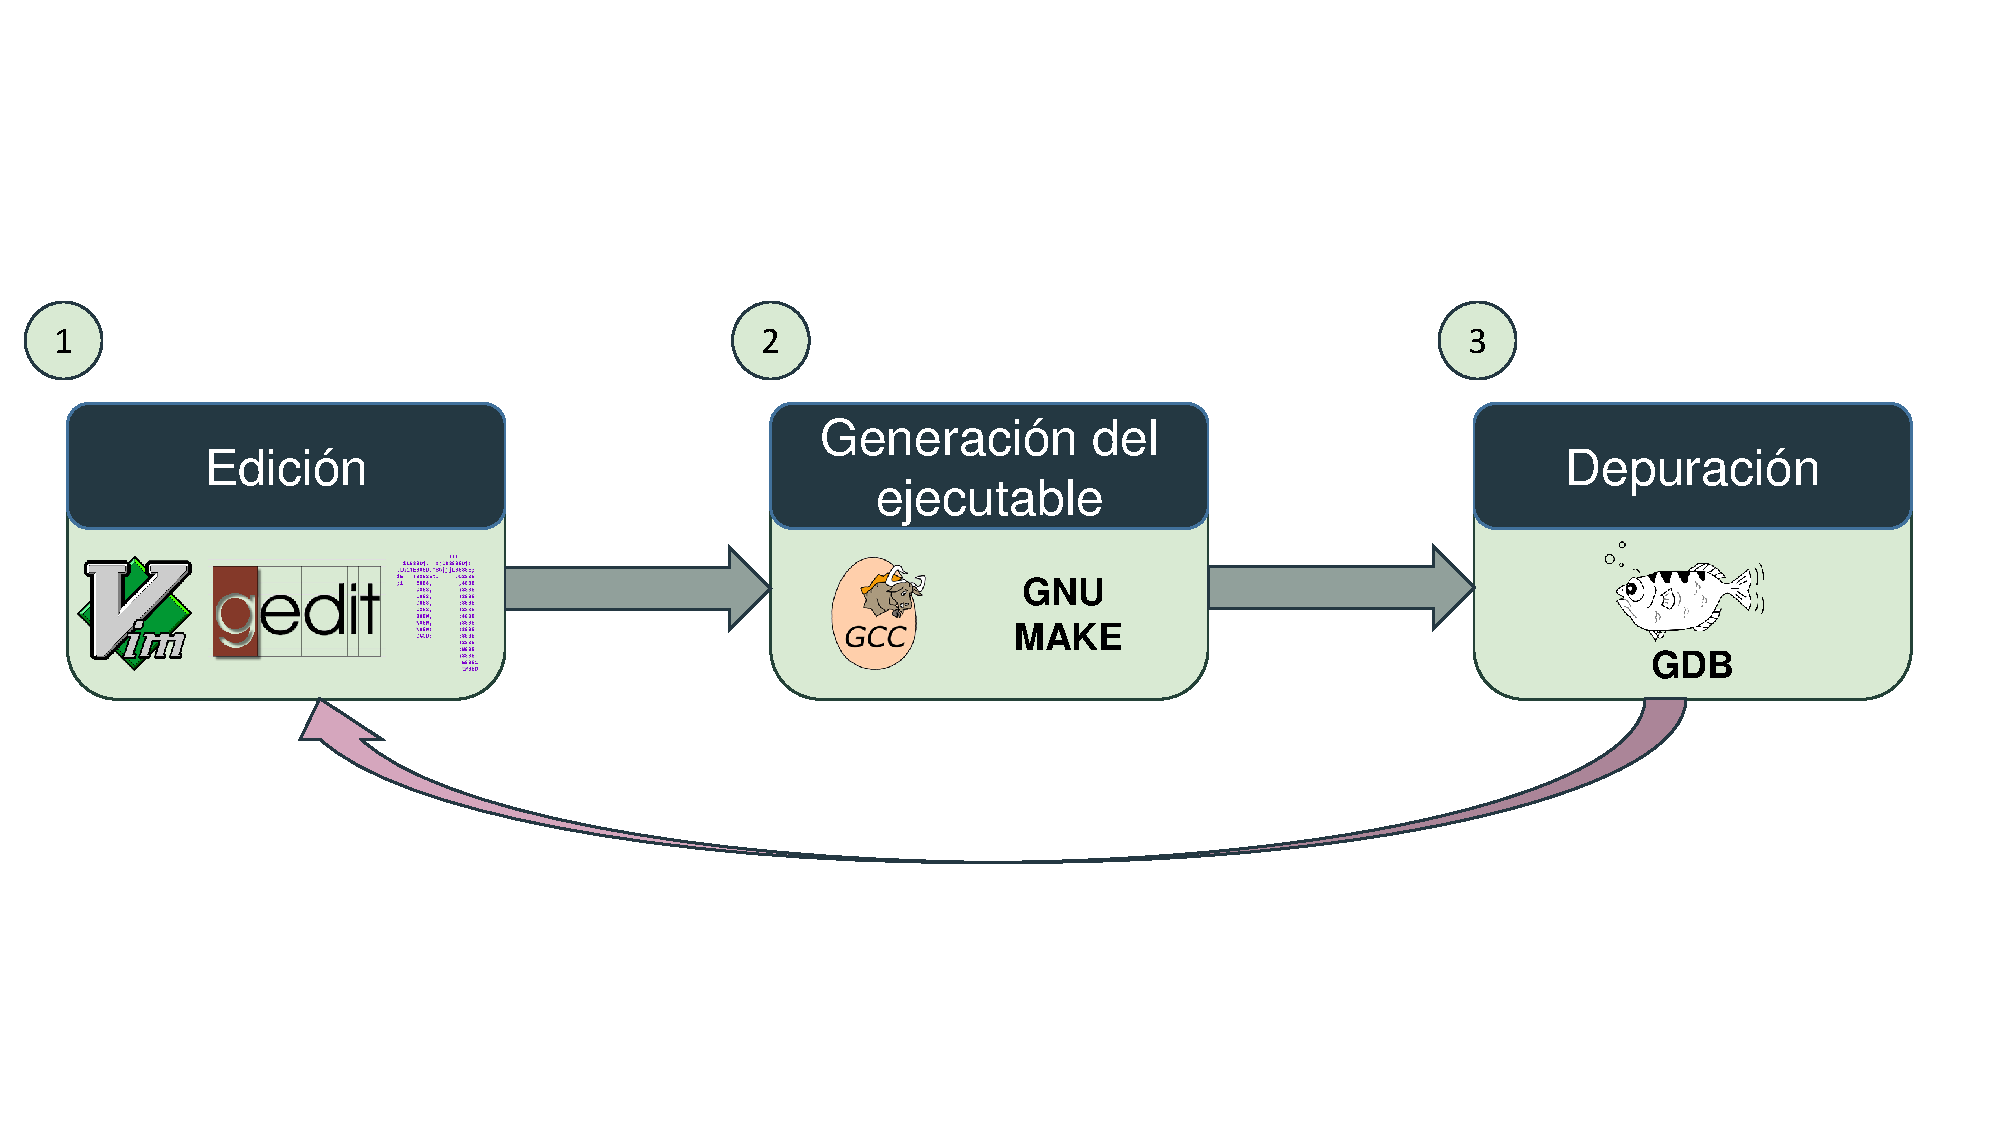
\includegraphics[trim={0.25cm 3cm 0 3cm}, clip, width=11cm, page=1]{figuras/Figuras.pdf}
			\par\end{centering}
	
			\caption{\label{FasesDesarrollo}Fases de desarrollo del ciclo de creación de un programa.}
		\end{figure}
	\end{frame}
	
	
	\begin{frame}{Generación del ejecutable}
		\setbeamercolor{block title}{use=structure,fg=white,bg=green!75!black}
		\setbeamercolor{block body}{use=structure,fg=black,bg=green!20!white}

		\vspace{-0.25cm}
		\begin{figure}
			\includegraphics[width=11cm, page=1]{figuras/generarejecutable.pdf}
		\end{figure}
	\end{frame}	
	
	\begin{frame}{Generación del ejecutable}
       \framesubtitle{Conjunto de herramientas GCC}
		\setbeamercolor{block title}{use=structure,fg=white,bg=green!75!black}
		\setbeamercolor{block body}{use=structure,fg=black,bg=green!20!white}

		\begin{figure}
			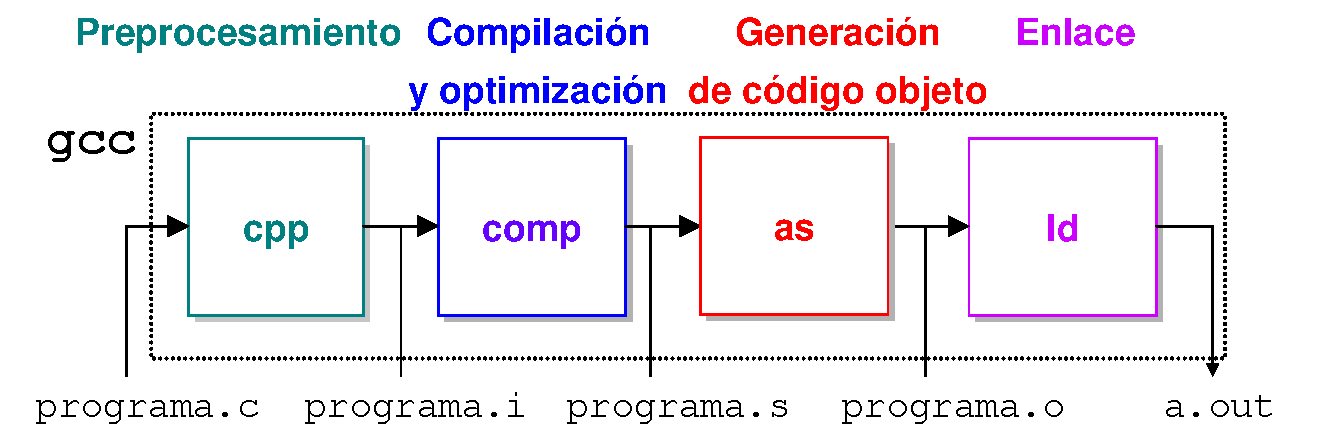
\includegraphics[width=11cm, page=1]{figuras/compilacionUnix.pdf}
		\end{figure}
		
		\begin{itemize}
			\item La orden \texttt{gcc} tiene opciones para generar los archivos intermedios	  (\texttt{-E, -S, -c}).
			\item Otras opciones de gcc: \texttt{-o, -Wall, -g}
		\end{itemize}
	\end{frame}	
	
	
	\begin{frame}{Generación del ejecutable}	
       \framesubtitle{Ejemplo de programa}
		\setbeamercolor{block title}{use=structure,fg=white,bg=green!75!black}
		\setbeamercolor{block body}{use=structure,fg=black,bg=green!20!white}
\vspace{-0.8cm}
\begin{minipage}[t]{0.55\textwidth}
		\lstinputlisting[  basicstyle=\scriptsize,  backgroundcolor=\color{gris}, keywordstyle=\bfseries\color{green!40!black},
language=c, frame=single, title=principal.c]{codigo/principal.c}
\end{minipage}		
\hspace{0.5cm}
\begin{minipage}[t]{0.4\textwidth}
		\lstinputlisting[  basicstyle=\scriptsize,
  backgroundcolor=\color{gris},
  keywordstyle=\bfseries\color{green!40!black},
language=c, frame=single, title=sumar.h]{codigo/sumar.h}
		\lstinputlisting[  basicstyle=\scriptsize,
  backgroundcolor=\color{gris},
  keywordstyle=\bfseries\color{green!40!black},
language=c, frame=single, title=sumar.c]{codigo/sumar.c}
\end{minipage}		
\vspace{-0.3cm}
\begin{itemize}
	\item \small{Proceso de generación del ejecutable programa:}
	\scriptsize{
	\begin{enumerate}
		\item \texttt{gcc -g -Wall -c principal.c}
		\item \texttt{gcc -g -Wall -c sumar.c}
		\item \texttt{gcc -g -Wall principal.o sumar.o -o programa}
	\end{enumerate}
}	
\end{itemize}

	\end{frame}

	\usebackgroundtemplate{\includegraphics[width=\paperwidth]{../../../../transparencias/comun/marcadeagua}}
	\begin{frame}{Generación del ejecutable}	
       \framesubtitle{Posibles avisos y errores al compilar con \texttt{gcc -Wall}}
		\setbeamercolor{block title}{use=structure,fg=white,bg=green!75!black}
		\setbeamercolor{block body}{use=structure,fg=black,bg=green!20!white}

\begin{footnotesize}
	\textbf{unused variable `\texttt{variable}'} \\
\begin{itemize}
\vspace{-0.2cm}
\justifying\item[]  Indica que \texttt{variable} se reserva y no se utiliza en todo el programa.
\end{itemize}

	\textbf{implicit declaration of function `\texttt{funcion}'} \\
\begin{itemize}
\vspace{-0.2cm}
\justifying\item[] Indica que no existe declaración previa a la llamada de \texttt{funcion}. Puede ser por varias causas, normalmente suele ser por la falta del archivo de cabecera correspondiente.
\end{itemize}


	\textbf{return type defaults to `int'} \\
\begin{itemize}
\vspace{-0.2cm}
\justifying\item[]  Indica que la función definida en esa línea no tiene explícitamente marcado el tipo de los datos que devuelve y se le asigna, por defecto, tipo entero.
\end{itemize}

	\textbf{suggest parentheses around assignment used as truth value} \\
\begin{itemize}
\vspace{-0.2cm}
\justifying\item[] Indica que se está realizando una asignación y una operación de comparación en la misma expresión o que se está realizando una asignación por error en lugar de una comparación, sugiriendo la utilización de paréntesis para asegurar que el orden de las dos operaciones es correcto.
\end{itemize}

	\end{footnotesize}	
	
\end{frame}


	\begin{frame}{Generación del ejecutable}	
       \framesubtitle{Posibles avisos y errores al compilar con \texttt{gcc -Wall}}
		\setbeamercolor{block title}{use=structure,fg=white,bg=green!75!black}
		\setbeamercolor{block body}{use=structure,fg=black,bg=green!20!white}

\begin{footnotesize}
	\textbf{return type of `main' is not `int'} \\
\begin{itemize}
\vspace{-0.2cm}
\justifying\item[]  Indica que el tipo devuelto por la función \texttt{main} no es un entero.
\end{itemize}

	\textbf{`return' with a value, in function returning void} \\
\begin{itemize}
\vspace{-0.2cm}
\justifying\item[] indica que se está devolviendo un valor desde una función declarada como \texttt{void}.
\end{itemize}

	\textbf{control reaches end of non-void function} \\
\begin{itemize}
\vspace{-0.2cm}
\justifying\item[]  Indica que se ha alcanzado el final de una función no declarada como \texttt{void} sin que se devuelva ningún valor.
\end{itemize}

	\textbf{assignment makes integer from pointer without a cast} \\
\begin{itemize}
\vspace{-0.2cm}
\justifying\item[] Indica que se está realizando una asignación entre valores de diferentes tipos sin utilizar conversiones cast.
\end{itemize}

	\end{footnotesize}	
	
\end{frame}



\section{Make}
	\begin{frame}{Make: Definición y características}
		\setbeamercolor{block title}{use=structure,fg=white,bg=green!75!black}
		\setbeamercolor{block body}{use=structure,fg=black,bg=green!20!white}
		\begin{block}{\textit{Make}}		
			\justifying Herramienta que permite automatizar la gestión de las órdenes de compilación y facilita la tarea de creación de ejecutables.		
		\end{block}		
		
		\begin{itemize}		
			\vfill\item \justifying Permite definir \textbf{una sola vez} las opciones de compilación de los módulos que forman parte del programa. \\
			\vfill\item \justifying Es capaz de llevar un \textbf{control de los cambios} que se han realizado en los archivos fuente y ejecutables.
			\vfill\item \justifying Se evita la recompilación de los módulos del programa que no hayan sido modificados y, por lo tanto, se optimiza el proceso de compilación.
		\end{itemize}
	\end{frame}
	
	\begin{frame}{Archivo \texttt{Makefile} (I): Definición y características}
		\setbeamercolor{block title}{use=structure,fg=white,bg=blue!75!black}
		\setbeamercolor{block body}{use=structure,fg=black,bg=blue!20!white}
		\begin{block}{Makefile}		
			\justifying Archivo de texto que utiliza \textit{make} para llevar a cabo la gestión de la compilación de programas. Este archivo contiene, en forma de reglas, las dependencias entre los diferentes archivos de un proyecto.	
		\end{block}		
		
		\begin{itemize}		
			\vfill\item \justifying Por defecto, la herramienta \textit{make} busca un archivo \texttt{makefile} o \texttt{Makefile} en el directorio actual. 
			\vfill\item \justifying Si se desea modificar este nombre, \textit{make} deberá invocarse con el parámetro -f seguido del nombre de archivo. \\
			\vfill\item \justifying Las reglas de un archivo \texttt{makefile} se ejecutan mediante una especie de \textit{backtracking}. La primera vez recorre las reglas hacia abajo y a continuación las resuelve de abajo hacia arriba.
		\end{itemize}
	\end{frame}	
	
	\begin{frame}{Archivo \texttt{Makefile} (II): Sintaxis y semántica}
		\lstinputlisting[language=c, frame=single, caption=Sintaxis de un \texttt{makefile}.]{codigo/makefile.txt}
		\begin{itemize}		
			\vfill\item \justifying \textbf{Objetivo}: Normalmente, es un archivo (o varios) que se quiere(n) crear o actualizar.
			\vfill\item \justifying \textbf{Dependencias}: Son nombres de archivos u otros objetivos necesarios para actualizar el objetivo de la regla.
			\vfill\item \justifying \textbf{orden\_{i}}: Orden necesaria para reconstruir el objetivo de la regla. Puede ser cualquier orden de la \textit{shell} o intérprete de órdenes. Debe comenzar necesariamente por el carácter <TAB> (tabulador).
		\end{itemize}
	\end{frame}	
	
	\begin{frame}{Archivo \texttt{Makefile} (III): Reglas ficticias}
		\setbeamercolor{block title}{use=structure,fg=white,bg=red!75!black}
		\setbeamercolor{block body}{use=structure,fg=black,bg=red!20!white}
		\begin{block}{Reglas ficticias}		
			\justifying Reglas que no generan un archivo específico sino que se utilizan para realizar una determinada tarea dentro del desarrollo de la aplicación. 
		\end{block}		
\vfill Para evitar confusiones entre el objetivo ficticio clean y un posible archivo que pueda existir con el mismo nombre, se suele utilizar el objetivo especial de tipo \texttt{PHONY}.
		\lstinputlisting[language=c, frame=single, caption=Sintaxis de un \texttt{makefile}.]{codigo/clean.txt}
	\end{frame}	

	\begin{frame}{Archivo \texttt{Makefile} (IV): Variables}
		\begin{itemize}		
			\vfill\item \justifying Las variables facilitan la portabilidad a diferentes plataformas y entornos así como la modificación del archivo \textit{makefile}.
			\vfill\item \justifying Las variables se suelen escribir en su totalidad en mayúsculas. 
			\vfill\item \justifying Para obtener el valor de una variable, se pone el signo '\$' y el nombre de la
variable entre paréntesis o llaves.
		\end{itemize}	
		\lstinputlisting[language=c, frame=single, caption=Sintaxis de un \texttt{makefile}.]{codigo/variables.txt}
	\end{frame}	
	
	\begin{frame}{Archivo \texttt{Makefile} (V): consejos para hacer un correcto \texttt{makefile}}
		\begin{itemize}
			\item ¿Expresiones repetidas frecuentemente? ¡\textbf{Usa variables}!
			\vfill\item Todo \texttt{makefile} comienza siempre por el objetivo principal. 
			\vfill\item ¿Tiene el objetivo todas sus dependencias? ¡\textbf{Revisa las relaciones entre los archivos}! 		
		\end{itemize}
	\end{frame}

	\begin{frame}{Archivo \texttt{Makefile} (VI): consejos para hacer un correcto \texttt{makefile}}
		\begin{itemize}
			
			\vfill\item Recuerda incluir los archivos de cabecera .h de los archivos creados cuando se vaya a crear la regla relacionada con el archivo objeto (.o). 			
			
			\vfill\item No olvides el \textit{clean}. Es tan importante como el resto de reglas.
		\end{itemize}
	\end{frame}


%\subsection{Ejemplos}
\subsection{Makefile correcto}
	\begin{frame}{Archivo \texttt{Makefile} (VII): cómo \textbf{SI} hacer un \texttt{makefile}}
		\lstinputlisting[language=c, frame=single, caption=Ejemplo de un \texttt{makefile}.]{codigo/makefile2.txt}
	\end{frame}	
	
\subsection{Makefile incorrecto}
	\begin{frame}{Archivo \texttt{Makefile} (VIII): cómo \textbf{NO} hacer un \texttt{makefile}}
\begin{bclogo}[arrondi=0.1,
    couleur=white, logo=\bcattention,
    ombre=true, couleurOmbre=gray!50, epOmbre=0.1, blur,
    barre=none, 
    ]{Errores típicos}{- Escribir una única regla. \\ - No emplear las dependencias en las órdenes.}
\end{bclogo}
		\lstinputlisting[language=c, frame=single, basicstyle=\small, caption=Ejemplo de un \texttt{makefile} INCORRECTO.]{codigo/makefile3.txt}

	\end{frame}	


\section{GDB}

	\begin{frame}{GDB: Definición y características}
		\setbeamercolor{block title}{use=structure,fg=white,bg=green!75!black}
		\setbeamercolor{block body}{use=structure,fg=black,bg=green!20!white}
		\begin{block}{\textit{GDB}}		
			\justifying Herramienta estándar de GNU que permite depurar un programa para mejorar su calidad.		
		\end{block}		
		
		\begin{itemize}		
			\vfill\item \justifying Es posible alterar y monitorizar los valores de las variables internas del programa. \\
			\vfill\item \justifying Es posible establecer puntos de ruptura para verificar el estado de ejecución del programa en un instante determinado.
			\vfill\item \justifying Permite encontrar fallos durante la ejecución del programa.
		\end{itemize}
	\end{frame}

\usebackgroundtemplate{}

	\begin{frame}{GDB: Definición y características}
		\setbeamercolor{block title}{use=structure,fg=white,bg=green!75!black}
		\setbeamercolor{block body}{use=structure,fg=black,bg=green!20!white}

%\begin{footnotesize}
%\begin{tabularx}{\textwidth}{CCCCCC}
%Ejecución                                  &                                                                   &                                                           & Variables y memoria                     &                                                                                                                            &                                                \\
%run                                        & \multicolumn{2}{c}{comenzar la ejecución del programa}                                                                        & print/format \textless item\textgreater &                                                                                                                            & imprimir un valor con formato                  \\
%set args \textless argumentos\textgreater  & \multicolumn{2}{c}{establecer los argumentos del programa}                                                                    & x/nfu \textless address\textgreater     &                                                                                                                            & volcado de n posiciones de memoria con formato \\
%quit                                       & \multicolumn{2}{c}{salir del depurador}                                                                                       & \textless item\textgreater              & \begin{tabular}[c]{@{}l@{}}expresión (e.g. nombre de variable) \\ dirección de memoria\\ $registro (e.g. $ax)\end{tabular} &                                                \\
%Puntos de ruptura                          &                                                                   &                                                           & format                                  & Formato                                                                                                                    &                                                \\
%break \textless position\textgreater       &                                                                   & establecer un punto de ruptura en una posición del código & a                                       & puntero                                                                                                                    &                                                \\
%delete \textless \# breakpoint\textgreater &                                                                   & borrar el punto de ruptura \#                             & d                                       & decimal con signo                                                                                                          &                                                \\
%clear                                      &                                                                   & ir a la siguiente ocurrencia                              & u                                       & decimal sin signo                                                                                                          &                                                \\
%Ejecución paso a paso                      &                                                                   &                                                           & f                                       & coma flotante                                                                                                              &                                                \\
%step                                       & ejecutar la siguiente línea de código entrando en las funciones   &                                                           & x                                       & hexadecimal                                                                                                                &                                                \\
%next                                       & ejecutar la siguiente línea de código sin entrar en las funciones &                                                           & b                                       & byte                                                                                                                       &                                                \\
%finish                                     & continuar hasta salir de la función actual                        &                                                           & w                                       & palabra (4 bytes)                                                                                                          &                                                \\
%continue                                   & continuar la ejecución del programa                               &                                                           & g                                       & palabra gigante (8 bytes)                                                                                                  &                                           
%\end{tabularx}
%
%\end{footnotesize}



		\begin{figure}
			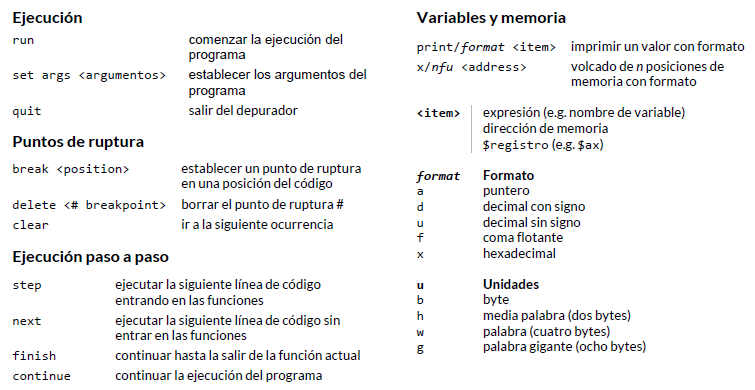
\includegraphics[width=\textwidth]{figuras/comandosGDB.PNG}
		\end{figure}
	\end{frame}

\usebackgroundtemplate{\includegraphics[width=\paperwidth]{../../../../transparencias/comun/marcadeagua}}



	\begin{frame}{Depuración con \texttt{GDB}}
	\lstinputlisting[language=c, frame=single, numbers=left, firstline=1, lastline=16, basicstyle=\footnotesize, backgroundcolor=\color{gris}, keywordstyle=\bfseries\color{green!40!black}, frame=single, title=\texttt{ejemplo\_gdb.c}]{codigo/ejemplo_gdb.c}
	\end{frame}	

	\begin{frame}{Depuración con \texttt{GDB}}
	\lstinputlisting[language=c, frame=single, numbers=left, firstline=16, firstnumber=16, lastline=30, basicstyle=\footnotesize, backgroundcolor=\color{gris}, keywordstyle=\bfseries\color{green!40!black}, frame=single, title=\texttt{ejemplo\_gdb.c} \textit{(cont.)}]{codigo/ejemplo_gdb.c}
	\end{frame}	
	
	\begin{frame}{Compilar, ejecutar y depurar \texttt{ejemplo\_gdb.c} (I)}
%	\begin{block}{}
	\footnotesize{
	\begin{enumerate}
	\item Compile el programa \texttt{ejemplo\_gdb.c}. 
	\item Ejecute el programa \texttt{ejemplo\_gdb.c} pasándole como parámetro \texttt{-l}. ¿Qué sucede?
	\item Compile el programa \texttt{ejemplo\_gdb.c} añadiendo el parámetro necesario para poder depurarlo.
	\item Inicie el depurador con el programa \texttt{ejemplo\_gdb}.
	\item Obtenga ayuda sobre las órdenes del depurador.
	\item Obtenga las funciones utilizadas por \texttt{ejemplo\_gdb}.
	\item Pase el parámetro \texttt{-l} al programa \texttt{ejemplo\_gdb}.
	\item Ejecute el programa \texttt{ejemplo\_gdb} ¿Qué sucede?
	\item Establezca tres puntos de ruptura: \textit{líneas 8} (\texttt{main}), \textit{17} y \textit{22}, respectivamente \footnote{\tiny{Establecer adecuadamente los puntos de ruptura es clave para acotar los errores de ejecución que se hayan producido y eliminarlos.}}.
	
	\seti
	\end{enumerate}
	}
%	\end{block}
	\end{frame}	
	
	\begin{frame}{Compilar, ejecutar y depurar \texttt{ejemplo\_gdb.c} (II)}
%	\begin{block}{}
	\footnotesize{
	\begin{enumerate}
	 \conti
	\item Ejecute \texttt{ejemplo\_gdb} hasta el primer punto de ruptura.
	\item Ejecutar la siguiente línea del programa (\textit{línea 12}).
	\item Ejecute las dos siguientes funciones (\texttt{printf}) \textbf{sin} entrar en su código.
	\item Ejecute la siguiente línea del programa (\texttt{for}).
	\item Muestre el valor de la variable \texttt{i}.
	\item Ejecute hasta el siguiente punto de ruptura (\textit{línea 22}).
	\item Ejecute hasta llegar a la segunda iteración del \texttt{for}. Si la línea es una función, ejecútela \textbf{sin} entrar en su código.
	\item Ejecute la línea del \texttt{for} (\textit{línea 17}).
	\item Imprima el valor de la variable \texttt{i} y el de \texttt{argv[2}]. Observe sus valores\ldots
	\item Ejecute la \textit{línea 19} sin entrar en el código de sus funciones. ¿Ha detectado cuál es el error?
	\seti
	\end{enumerate}
	}
%	\end{block}
	\end{frame}	

\end{document}


